
\documentclass[12pt, tikz, border=5mm]{standalone}
\usepackage{tikz}
\begin{document}
\usetikzlibrary{quotes,angles}
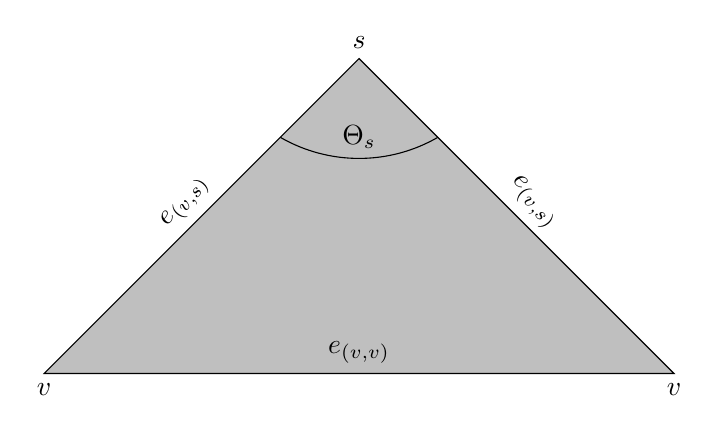
\begin{tikzpicture}
  
  

  
\draw[fill=gray!50]   (0,0) coordinate[label=below:$v$] (a) -- node[above,rotate=50] {$e_{(v,s)}$} 
        (4,4) coordinate[label=above:$s$] (b) -- node[above,rotate=-50] {$e_{(v,s)}$}
        (8,0) coordinate[label=below:$v$] (c) --node[above] {$e_{(v,v)}$}  cycle;
        
    \draw[fill=gray!50]  ({4+1},{4-1}) arc (-60:-120:2) node[above,midway]{$\Theta_{s}$};
    
    
%\pic[draw=orange,fill=teal!30,angle radius=7mm,angle eccentricity=1.4,right,inner sep=1pt,font=\footnotesize ,"$\Theta_{s}$"] {angle = a--b--c};

\end{tikzpicture}
\end{document}